\documentclass{fmbvecto}

\usepackage[spanish]{babel}
\usepackage{caption}

\renewcommand{\title}{Ejemplo de solución correcta del taller 2}
\newcommand{\subject}{Cálculo Vectorial}

\renewcommand{\labelenumii}{\theenumii}
\renewcommand{\theenumii}{\theenumi.\arabic{enumii}.}

\NewDocumentCommand{\itemp}{o}{\item (#1 puntos)}


\begin{document}

Miércoles, 10 de julio de 2024

\begin{center}
    \textbf{\LARGE \title} \\
    {\large \subject}
\end{center}


Profesor: Jacinto Eloy Puig Portal, \href{mailto:jpuig@uniandes.edu.co}{jpuig@uniandes.edu.co}. \\
Monitor: Federico Melo Barrero, \href{mailto:f.melo@uniandes.edu.co}{f.melo@uniandes.edu.co}.\\

\textbf{\Large Preámbulo}

Las instrucciones referentes a la entrega del taller están escritas en \href{https://bloqueneon.uniandes.edu.co/d2l/home}{Bloque Neón}.

\subsection*{Bonos}
\begin{itemize}
  \item Se sumarán 0.25 puntos de bonificación a la nota del taller si su contenido está ordenado y puede leerse con facilidad.
  \item Se sumarán 0.25 puntos de bonificación a la nota del taller si no contiene errores léxicos, gramaticales ni faltas de ortografía.
\end{itemize}
La nota del taller puede exceder el 5.0.

\subsection*{Recomendaciones}

No necesita hacer uso de herramientas que le ayuden a hacer matemáticas, ya sean calculadoras, aplicaciones, grandes modelos de lenguaje u otras. Le recomiendo que no lo haga

Recuerde incluir las unidades siempre que trate con magnitudes físicas.

\section{Taller 1}

\begin{problema}[Corrección del taller 1]
    
    (1 punto) Corrija todos los errores que tuvo su grupo en el taller 1. Si no tuvo errores, omita este punto.

    \tcblower
    
    En este punto simplemente revisaré que se hayan corregido los errores y abordado los comentarios que dejé en su taller. Naturalmente, la corrección debe ser correcta, sobretodo teniendo en cuenta que el solucionario del taller 1 está en Bloque Neón desde el domingo 23 de junio.

\end{problema}

\section{Integrales dobles}

\begin{problema}[Integral doble en región de tipo 3]
    
    (1 punto) Calcule analíticamente la integral \[ \int_{1}^{2} \int_{0}^{\ln y} (y-1) \sqrt{1 + \mathrm{e}^{2x}} \: \mathrm{d}x \: \mathrm{d}y. \] No utilice aproximaciones numéricas ni herramientas computacionales. No omita ningún paso en su solución.

\tcblower
\textbf{Solución:}

    \subsection{Cambiar el orden de integración}

    Antes de calcular una integral doble, siempre vale la pena inspeccionar la región sobre la que se integra, pues si la región resulta ser de tipo 3, se puede cambiar el orden de integración, lo cual puede facilitar o incluso posibilitar el cálculo de la integral. Para ello, es recomendable hacer un bosquejo de la región. \\
    
    Sea \(D\) la región de integración y \(f(x, y)\) el integrando, de forma que \[ \int_D f = \int_{1}^{2} \int_{0}^{\ln y} (y-1) \sqrt{1 + \mathrm{e}^{2x}} \: \mathrm{d}x \: \mathrm{d}y. \]
    La región \(D\), expresada como región de tipo 2, es el conjunto
    \[D = \{(x, y) | 0 \leq x \leq \ln y \ \land \ 1 \leq y \leq 2\}.\]
    Un bosquejo de la región se muestra en la figura \ref{fig:region-tipo-3}.

    \begin{center}
        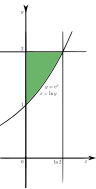
\includegraphics[width=0.4\textwidth]{region-tipo-3.png}
        \captionof{figure}{Región de integración \(D\).}
        \label{fig:region-tipo-3}
    \end{center}

    \vspace{1em}
    A partir del bosquejo, resulta evidente que \(D\) efectivamente es una región de tipo 3, pues también se puede expresar como región de tipo 1, delimitada por un intervalo numérico en el eje \(x\) y por curvas continuas en el eje \(y\). Se expresa la curva \(x = \ln y\) como \(y = \mathrm{e}^x\), de forma que \(D\) se puede expresar como
    \[D = \{(x, y) | 0 \leq x \leq \ln 2 \ \land \ \mathrm{e}^x \leq y \leq 2\}.\]
    Por lo tanto, la integral se puede reescribir como
    \[ \int_D f = \int_{0}^{\ln 2} \int_{\mathrm{e}^x}^{2} (y-1) \sqrt{1 + \mathrm{e}^{2x}} \: \mathrm{d}y \: \mathrm{d}x. \]

    A partir del proceso anterior, se tienen dos formas de expresar la misma integral. Ahora, se debe ponderar cuál forma es la más conveniente para calcular la integral. En la primera forma, la integral interna es
    \[ \int_{0}^{\ln y} \sqrt{1 + \mathrm{e}^{2x}} \: \mathrm{d}x, \]
    mientras que en la segunda forma, la integral interna es
    \[ \int_{\mathrm{e}^x}^{2} (y-1) \: \mathrm{d}y. \]
    Resulta evidente que es mucho más sencillo calcular la integral en la segunda forma.

    \subsection{Calcular la integral doble}

    Con eso en mente, se procede a calcular la integral.
    \begin{align*}
        \int_D f &= \int_{0}^{\ln 2} \int_{\mathrm{e}^x}^{2} (y-1) \sqrt{1 + \mathrm{e}^{2x}} \: \mathrm{d}y \: \mathrm{d}x \\
        &= \int_{0}^{\ln 2} \sqrt{1 + \mathrm{e}^{2x}} \left( \int_{\mathrm{e}^x}^{2} (y-1) \: \mathrm{d}y \right) \mathrm{d}x \\
        &= \int_{0}^{\ln 2} \sqrt{1 + \mathrm{e}^{2x}} \left( \int_{\mathrm{e}^x}^{2} y \: \mathrm{d}y - \int_{\mathrm{e}^x}^{2} 1 \: \mathrm{d}y \right) \mathrm{d}x \\
        &= \int_{0}^{\ln 2} \sqrt{1 + \mathrm{e}^{2x}} \left( \left. \frac{y^2}{2} \right\vert_{\mathrm{e}^x}^{2} -  1(2 - \mathrm{e}^x) \right) \mathrm{d}x \\
        &= \int_{0}^{\ln 2} \sqrt{1 + \mathrm{e}^{2x}} \left( \frac{2^2}{2} - \frac{(\mathrm{e}^x)^2}{2} - 2 + \mathrm{e}^x \right) \mathrm{d}x \\
        &= \int_{0}^{\ln 2} \sqrt{1 + \mathrm{e}^{2x}} \left( 2 - \frac{\mathrm{e}^{2x}}{2} - 2 + \mathrm{e}^x \right) \mathrm{d}x \\
        &= \int_{0}^{\ln 2} \sqrt{1 + \mathrm{e}^{2x}} \left( \mathrm{e}^x - \frac{\mathrm{e}^{2x}}{2}\right) \mathrm{d}x \\
        &= \int_{0}^{\ln 2} \mathrm{e}^x \sqrt{1 + \mathrm{e}^{2x}} - \frac{\mathrm{e}^{2x}}{2} \sqrt{1 + \mathrm{e}^{2x}} \mathrm{d}x \\
        &= \int_{0}^{\ln 2} \mathrm{e}^x \sqrt{1 + \mathrm{e}^{2x}} \: \mathrm{d}x  - \int_{0}^{\ln 2} \frac{\mathrm{e}^{2x}}{2} \sqrt{1 + \mathrm{e}^{2x}} \: \mathrm{d}x \\
        &= I_1  - I_2.
    \end{align*}

    \subsection{Calcular la integral \(I_1\)}

    Para evaluar \(I_1\) tuve que utilizar tres técnicas de integración: primero, utilizo sustitución simple; luego, sustitución trigonométrica; por último, integración por partes. Además, para reemplazar los valores, me ayudo de un poco de trigonometría. Posiblemente exista un método más elegante o breve para evaluar esta integral, sin embargo, presento este, que utiliza técnicas básicas que vieron en el curso de Cálculo Integral. \\
    
    Como primer paso para evaluar \(I_1\), se realiza el cambio de variable \(u = \mathrm{e}^{x}\), de forma que \(\mathrm{d}u = \mathrm{e}^{x} \: \mathrm{d}x\). Se deben modificar también los límites de integración: para el límite superior, se tiene \(u = \mathrm{e}^{\ln 2} = 2\); para el límite inferior, se tiene \(u = \mathrm{e}^{0} = 1\). Por lo tanto,
    \[ I_1 = \int_{0}^{\ln 2} \mathrm{e}^x \sqrt{1 + \mathrm{e}^{2x}} \: \mathrm{d}x = \int_{1}^{2} \sqrt{1 + u^2} \: \mathrm{d}u. \]
    Lo anterior es una integral de una variable con una suma de cuadrados dentro de un radical. Ergo, es natural usar sustitución trigonométrica para resolverla. Se realiza el cambio de variable \(u = \tan \theta\), de forma que \(\mathrm{d}u = \sec^2 \theta \: \mathrm{d}\theta\). Se deben modificar también los límites de integración: para el límite inferior, se tiene \(\theta = \arctan 1 = \frac{\pi}{4}\); para el límite superior, se tiene \(\theta = \arctan 2\). Por lo tanto,
    \begin{align*}
        I_1 &= \int_{1}^{2} \sqrt{1 + u^2} \: \mathrm{d}u \\
        &= \int_{\frac{\pi}{4}}^{\arctan 2} \sqrt{1 + \tan^2 \theta} \sec^2 \theta \: \mathrm{d}\theta \\
        &= \int_{\frac{\pi}{4}}^{\arctan 2} \sqrt{\sec^2 \theta} \sec^2 \theta \: \mathrm{d}\theta \\
        &= \int_{\frac{\pi}{4}}^{\arctan 2} \sec^3 \theta \: \mathrm{d}\theta.
    \end{align*}
    Para evaluar la integral de secante cúbica, una opción es expresarla como el producto \(\sec^3 \theta = \sec^2 \theta \sec \theta\) y usar integración por partes. En pos de la simplicidad, se evaluará como integral indefinida. Recuérdese la fórmula de integración por partes,
    \[ \int u \: \mathrm{d}v = uv - \int v \: \mathrm{d}u. \]
    Se elige \(u = \sec \theta\) y \(\mathrm{d}v = \sec^2 \theta \: \mathrm{d}\theta\), pensando en sacar provecho de que \(\der[][\theta] \tan \theta = \sec^2 \theta\). Se tiene entonces que \(\mathrm{d}u = \sec \theta \tan \theta \: \mathrm{d}\theta\) y \(v = \tan \theta\). Por lo tanto,
    \begin{align*}
        \int \sec^3 \theta \: \mathrm{d}\theta &= \sec \theta \tan \theta  - \int \tan \theta \sec \theta \tan \theta \: \mathrm{d}\theta \\
        &=  \sec \theta \tan \theta  - \int \sec \theta \tan^2 \theta \: \mathrm{d}\theta \\
        &=  \sec \theta \tan \theta  - \int \sec \theta (\sec^2 \theta - 1)\: \mathrm{d}\theta \\
        &=  \sec \theta \tan \theta  - \int \sec^3 \theta - \sec \theta \: \mathrm{d}\theta \\
        &=  \sec \theta \tan \theta  - \int \sec^3 \theta \: \mathrm{d}\theta + \int \sec \theta \: \mathrm{d}\theta \\
        2 \int \sec^3 \theta \: \mathrm{d}\theta &= \sec \theta \tan \theta + \int \sec \theta \: \mathrm{d}\theta \\
        \int \sec^3 \theta \: \mathrm{d}\theta &= \frac{1}{2} \sec \theta \tan \theta + \frac{1}{2} \ln |\sec \theta + \tan \theta| + C.
    \end{align*}
    En ese último paso, la integral de \(\sec \theta\) es conocida. Si no la recuerda, se calcula multiplicando el integrando por \(\frac{\sec \theta + \tan \theta}{\sec \theta + \tan \theta}\) para obtener una integral de la forma \(\indint{\frac{f'(x)}{f(x)}}[x] = \ln \abs{f(x)} + C\). Con eso, se tiene el valor de la integral de secante cúbico, que se puede reemplazar en la integral \(I_1\) para obtener su valor.
    \begin{align*}
        I_1 =& \int_{\frac{\pi}{4}}^{\arctan 2} \sec^3 \theta \: \mathrm{d}\theta \\
        =& \frac{1}{2} \sec \theta \tan \theta + \frac{1}{2} \ln |\sec \theta + \tan \theta| \Bigg\vert_{\frac{\pi}{4}}^{\arctan 2} \\
        =& \frac{1}{2} \sec (\arctan 2) \tan (\arctan 2) + \frac{1}{2} \ln |\sec (\arctan 2) + \tan( \arctan 2)| \\ &- \frac{1}{2} \sec \frac{\pi}{4} \tan \frac{\pi}{4} - \frac{1}{2} \ln \left|\sec \frac{\pi}{4} + \tan \frac{\pi}{4}\right|
    \end{align*}
    Para calcular los valores, note que, por trigonometría:
    \begin{itemize}
        \item \(\sec \frac{\pi}{4} = \sqrt{2}\),
        \item \(\tan \frac{\pi}{4} = 1\),
        \item \(\sec (\arctan 2) = \sqrt{1 + 2^2} = \sqrt{5}\),
        \item \(\tan (\arctan 2) = 2\).
    \end{itemize}
    Si no lo recuerda, puede hacer dos cosas: primero, dibujar un triángulo rectángulo con ángulo de \(\frac{\pi}{4}\) radianes y catetos de longitud 1, para percatarse de que la hipotenusa tendrá longitud \(\sqrt{2}\); segundo, convencerse de que \(\tan (\arctan x) = x\) y \(\sec (\arctan x) = \sqrt{1 + x^2}\), lo cual se puede deducir manipulando cualquier triángulo rectángulo. \\
    
    Reemplazando los valores anteriores en la expresión para \(I_1\), se tiene que
    \begin{align*}
        I_1 =& \frac{1}{2} \sqrt{5} \cdot 2 + \frac{1}{2} \ln |\sqrt{5} + 2| - \frac{1}{2} \sqrt{2} \cdot 1 - \frac{1}{2} \ln |\sqrt{2} + 1| \\
        =& \sqrt{5} + \frac{\ln(\sqrt{5} + 2)}{2}  - \frac{\sqrt{2}}{2}  - \frac{\ln(\sqrt{2} + 1)}{2}.
    \end{align*}

    \subsection{Calcular la integral \(I_2\)}

    Para evaluar \(I_2\), se realiza un cambio de variable similar al anterior, \(u = \mathrm{e}^{2x}\). Así, \(\mathrm{d}u = 2 \mathrm{e}^{2x} \: \mathrm{d}x\), y los límites de integración se modifican de la siguiente manera: para el límite superior, se tiene \(u = \mathrm{e}^{2 \ln 2} = 4\); para el límite inferior, se tiene \(u = \mathrm{e}^{2 \cdot 0} = 1\). Por lo tanto,
    \[ I_2 = \int_{0}^{\ln 2} \frac{\mathrm{e}^{2x}}{2} \sqrt{1 + \mathrm{e}^{2x}} \: \mathrm{d}x = \frac{1}{4} \int_{1}^{4} \sqrt{1 + u} \: \mathrm{d}u. \]
    Aunque esta integral se asemeja superficialmente a la anterior, note que la expresión dentro del radicando es una función lineal. Esto hace que integrarla sea muchísimo más fácil. Basta con la sustitución \(v = 1 + u\), de forma que \(\mathrm{d}v = \mathrm{d}u\). Cambiar los límites de integración es trivial: para el límite inferior, se tiene \(v = 1 + 1 = 2\); para el límite superior, se tiene \(v = 1 + 4 = 5\). Así pues,
    \begin{align*}
        I_2 &= \frac{1}{4} \int_{1}^{4} \sqrt{1 + u} \: \mathrm{d}u \\
        &= \frac{1}{4} \int_{2}^{5} \sqrt{v} \: \mathrm{d}v \\
        &= \frac{1}{4} \left. \frac{2}{3} v^{3/2} \right\vert_{2}^{5} \\
        &= \frac{1}{6} \left( 5^{3/2} - 2^{3/2} \right) \\
        &= \frac{5 \sqrt{5} - 2 \sqrt{2}}{6}.
    \end{align*}

    \subsection{Concluir}

    Finalmente, se reemplazan los valores de \(I_1\) e \(I_2\) en la expresión para la integral original, \(I_1 - I_2\), para obtener el valor de la integral original.
    \begin{align*}
        \int_D f &= I_1 - I_2 \\
        &= \sqrt{5} + \frac{\ln(\sqrt{5} + 2)}{2}  - \frac{\sqrt{2}}{2}  - \frac{\ln(\sqrt{2} + 1)}{2} - \frac{5 \sqrt{5} - 2 \sqrt{2}}{6}.
    \end{align*}
\end{problema}

\section{Integrales triples}

\begin{problema}[Masa y centro de masa]
    
    (1 punto) Considere los paraboloides \(z = 10 - x^2 - y^2\) y \(z = 6 + x^2 + y^2\). Suponga que \(R\) es el sólido cuya forma está dada por la región encerrada por esos paraboloides. Si \(R\) presenta una densidad uniforme de \(8 \: \text{kg} \: \text{m}^{-3}\), indique cuál es la masa de \(R\) y cuál es la coordenada \(z\) de su centro de masa.
\tcblower
\textbf{Solución:}\\

Primeramente, es importante identificar las herramientas matemáticas que se necesitan para resolver este problema. En esencia, se busca calcular la masa y el centro de masa de un sólido \(R\) con densidad uniforme. Para ello, resulta útil recordar que tanto la masa como el centro de masa se pueden calcular mediante integrales triples sobre el sólido. En particular, la masa de un sólido con densidad uniforme se puede calcular mediante la integral,
\[m_R = \int_{R} \rho(x,y,z) \: \mathrm{d}x \: \mathrm{d}y \: \mathrm{d}z,\]
y la coordenada \(z\) del centro de masa, que denoto por \(\bar{z}\), se puede calcular mediante la integral,
\[\bar{z} = \frac{\int_{R} z\rho(x,y,z) \: \mathrm{d}x \: \mathrm{d}y \: \mathrm{d}z}{\int_{R} \rho(x,y,z) \: \mathrm{d}x \: \mathrm{d}y \: \mathrm{d}z}.\]
\vspace*{1em}

Con eso en mente, un prerrequisito para plantear las integrales es poder describir la región tridimensional encerrada por los dos paraboloides. Para ello, resulta útil hacer un bosquejo de la región. Es fácil imaginarse las gráficas si se da cuenta de que ambos paraboloides son traslaciones del paraboloide \(z = x^2 + y^2\) en el eje \(z\). En particular, el paraboloide \(z = 6 + x^2 + y^2\) es una traslación de \(z = x^2 + y^2\) en \(z = 6\), mientras que el paraboloide \(z = 10 - (x^2 + y^2)\) es una traslación de \(z = -(x^2 + y^2)\), el paraboloide que abre hacia abajo, en \(z = 10\). Eso permite llegar rápidamente a un bosquejo de la región como el que se muestra en la figura \ref{fig:interseccion-paraboloides}.

\begin{center}
    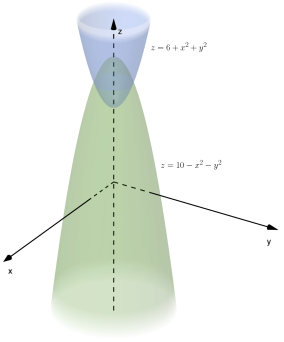
\includegraphics[width=0.6\textwidth]{interseccion-paraboloides.png}
    \captionof{figure}{Región encerrada por los paraboloides \(z = 10 - x^2 - y^2\) y \(z = 6 + x^2 + y^2\).}
    \label{fig:interseccion-paraboloides}
\end{center}
\vspace*{1em}
Resulta evidente que la región presenta simetría cilíndrica con respecto al eje \(z\). Por ende, será más sencillo describir la región mediante coordenadas cilíndricas. En coordenadas cilíndricas, note que:
\begin{itemize}
    \item El paraboloide \(z = 10 - x^2 - y^2\) se expresa como \(z = 10 - r^2\). Recuerde que el radio polar está dado por el teorema de Pitágoras como \(r = \sqrt{x^2 + y^2}\).
    \item El paraboloide \(z = 6 + x^2 + y^2\) se expresa como \(z = 6 + r^2\).
\end{itemize}
\vspace*{1em}
Para definir la región \(R\) en coordenadas cilíndricas, note que:
\begin{itemize}
    \item El ángulo polar \(\theta\) varía en el intervalo \([0, 2\uppi]\), pues la región recorre una revolución completa en torno al eje \(z\).
    \item El radio polar \(r\) varía en el intervalo \([0, r_0]\), donde \(r_0\) es el radio de la intersección entre los dos paraboloides. Para hallar la intersección de los paraboloides, se igualan sus ecuaciones:
    \begin{align*}
        10 - x^2 - y^2 &= 6 + x^2 + y^2 \\
        4 &= 2x^2 + 2y^2 \\
        2 &= x^2 + y^2.
    \end{align*}
    La ecuación resultante tiene una forma muy familiar, a saber, \(x^2+y^2 = r^2\), que es la ecuación de un círculo con radio \(r\) centrado en el origen. Así, la intersección entre los dos paraboloides es el círculo de radio \(\sqrt{2}\) centrado en el origen. Por consiguiente, la región \(r\) varía en el intervalo \([0, \sqrt{2}]\).
    \item La coordenada \(z\) varía en el intervalo \([6 + r^2, 10 - r^2]\), pues la región está encerrada entre los dos paraboloides.
\end{itemize}
A partir de eso, se puede describir la región encerrada por los dos paraboloides en coordenadas polares como
\[R = \{(r, \theta, z) | 0 \leq \theta \leq 2\uppi \ \land \ 0 \leq r \leq \sqrt{2} \ \land \ 6 + r^2 \leq z \leq 10 - r^2\}.\]
Solo queda pendiente un detalle para plantear la integral de la masa y el centro de masa: recordar que, al realizar un cambio de coordenadas, se debe incluir en la integral una medida de la distorsión del volumen a causa de la transformación. Dicha medida es el valor absoluto del jacobiano, que para las coordenadas cilíndricas es \(r\). Lo puede calcular como el determinante de la matriz de derivadas parciales de la función de transformación de coordenadas (pero le sugiero que, por lo menos durante este curso, ¡se sepa los jacobianos comunes de memoria!).\\

Teniendo todo eso en cuenta, la integral de la masa se puede plantear como
\[m_R = \int_{0}^{2\uppi} \int_{0}^{\sqrt{2}} \int_{6 + r^2}^{10 - r^2} 8 \: r \: \mathrm{d}z \: \mathrm{d}r \: \mathrm{d}\theta.\]

Por otro lado, la integral de la coordenada \(z\) del centro de masa se puede plantear como
\[\bar{z} = \frac{\int_{0}^{2\uppi} \int_{0}^{\sqrt{2}} \int_{6 + r^2}^{10 - r^2} z \cdot 8 \: r \: \mathrm{d}z \: \mathrm{d}r \: \mathrm{d}\theta}{\int_{0}^{2\uppi} \int_{0}^{\sqrt{2}} \int_{6 + r^2}^{10 - r^2} 8 \: r \: \mathrm{d}z \: \mathrm{d}r \: \mathrm{d}\theta}.\]

Ambas son integrales triples muy sencillas. Calculo primero la integral correspondiente a la masa:
\begin{align*}
    m_R &= \int_{0}^{2\uppi} \int_{0}^{\sqrt{2}} \int_{6 + r^2}^{10 - r^2} 8 \: r \: \mathrm{d}z \: \mathrm{d}r \: \mathrm{d}\theta \\
    &= 8 \int_{0}^{2\uppi} \int_{0}^{\sqrt{2}} \left. z \right\vert_{6 + r^2}^{10 - r^2} \: r \: \mathrm{d}r \: \mathrm{d}\theta \\
    &= 8 \int_{0}^{2\uppi} \int_{0}^{\sqrt{2}} (10 - r^2 - 6 - r^2) \: r \: \mathrm{d}r \: \mathrm{d}\theta \\
    &= 8 \int_{0}^{2\uppi} \int_{0}^{\sqrt{2}} (4 - 2r^2) \: r \: \mathrm{d}r \: \mathrm{d}\theta \\
    &= 8 \int_{0}^{2\uppi} \int_{0}^{\sqrt{2}} (4r - 2r^3) \: \mathrm{d}r \: \mathrm{d}\theta \\
    &= 8 \int_{0}^{2\uppi} \left. \left(2r^2 - \frac{2r^4}{4}\right) \right\vert_{0}^{\sqrt{2}} \: \mathrm{d}\theta \\
    &= 8 \int_{0}^{2\uppi} \left(2 \cdot 2 - \frac{2 \cdot 2^2}{4}\right) \: \mathrm{d}\theta \\
    &= 8 \int_{0}^{2\uppi} (4 - 2) \: \mathrm{d}\theta \\
    &= 8 \int_{0}^{2\uppi} 2 \: \mathrm{d}\theta \\
    &= 8 \cdot 2 \cdot \left.\theta \right\vert_{0}^{2\uppi} \\
    &= 8 \cdot 2 \cdot 2\uppi \\
    &= 32\uppi.
\end{align*}

Con eso, se llega a la primera conclusión:
\begin{gbox}
    La masa del sólido \(R\) es de \(32\uppi \: \text{kg}\).
\end{gbox}
\vspace*{1em}
Ahora, antes de calcular la integral de la coordenada \(z\) del centro de masa, quiero mencionar que muchas veces en matemática, vale la pena frenar y pensar en caminos alternativos para el problema. Fortuitamente, este es un ejemplo de problema en el cual, si piensa fuera de la caja, puede hallar una idea que le permite ahorrarse el cálculo por completo.

\vspace*{1em}
Recordará de sus clases de Física 1 que, si un sólido tiene densidad uniforme, entonces su centro de masa coincide con su centroide geométrico. El centroide geométrico de la región en cuestión es particularmente fácil de hallar, por dos razones:
\begin{itemize}
    \item La región es simétrica con respecto al plano \(z = 8\), que es el punto medio entre las alturas de los dos paraboloides. Para darse cuenta de esto, note que, como ya se mencionó, ambos paraboloides tienen forma idéntica: solo difieren en su altura y en la dirección en la que abren. Como uno abre hacia arriba en \(z = 6\) y el otro hacia abajo en \(z = 10\), la mitad de la figura en el eje \(z\) tendrá que ser el punto medio entre esas dos alturas, \(z = 8\).
    \item Para un sólido con simetría cilíndrica, naturalmente el centroide geométrico estará en su eje de simetría. En este caso, el eje de simetría es el eje \(z\).
\end{itemize}
Ergo, el centroide geométrico, que en este caso es también el centro de masa, es el punto \((0, 0, 8)\). Con eso, se llega a la segunda conclusión sin necesidad alguna de cálculo vectorial:
\begin{gbox}
    La coordenada \(z\) del centro de masa del sólido \(R\) es \(8\).
\end{gbox}

Por completitud, y para demostrar que el ejercicio es perfectamente factible sin tener presente ese detalle propio de la física, a continuación hago el cálculo de la integral de la coordenada \(z\) del centro de masa:

\begin{align*}
    \bar{z} &= \frac{\int_{0}^{2\uppi} \int_{0}^{\sqrt{2}} \int_{6 + r^2}^{10 - r^2} z \cdot 8 \: r \: \mathrm{d}z \: \mathrm{d}r \: \mathrm{d}\theta}{\int_{0}^{2\uppi} \int_{0}^{\sqrt{2}} \int_{6 + r^2}^{10 - r^2} 8 \: r \: \mathrm{d}z \: \mathrm{d}r \: \mathrm{d}\theta} \\
    &= \frac{8 \int_{0}^{2\uppi} \int_{0}^{\sqrt{2}} \left. \frac{z^2}{2} \right\vert_{6 + r^2}^{10 - r^2} \: r \: \mathrm{d}r \: \mathrm{d}\theta}{32\uppi} \\
    &= \frac{8 \int_{0}^{2\uppi} \int_{0}^{\sqrt{2}} \left( \frac{(10 - r^2)^2}{2} - \frac{(6 + r^2)^2}{2} \right) \: r \: \mathrm{d}r \: \mathrm{d}\theta}{32\uppi} \\
    &= \frac{8 \int_{0}^{2\uppi} \int_{0}^{\sqrt{2}} \left( \frac{100 - 20r^2 + r^4}{2} - \frac{36 + 12r^2 + r^4}{2} \right) \: r \: \mathrm{d}r \: \mathrm{d}\theta}{32\uppi} \\
    &= \frac{8 \int_{0}^{2\uppi} \int_{0}^{\sqrt{2}} \left( \frac{64 - 32r^2}{2} \right) \: r \: \mathrm{d}r \: \mathrm{d}\theta}{32\uppi} \\
    &= \frac{8 \int_{0}^{2\uppi} \int_{0}^{\sqrt{2}} (32r - 16r^3) \: \mathrm{d}r \: \mathrm{d}\theta}{32\uppi} \\
    &= \frac{8 \int_{0}^{2\uppi} \left. (16r^2 - 4r^4) \right\vert_{0}^{\sqrt{2}} \: \mathrm{d}\theta}{32\uppi} \\
    &= \frac{8 \int_{0}^{2\uppi} (16 \cdot 2 - 4 \cdot 2^2) \: \mathrm{d}\theta}{32\uppi} \\
    &= \frac{8 \int_{0}^{2\uppi} (32 - 16) \: \mathrm{d}\theta}{32\uppi} \\
    &= \frac{8 \int_{0}^{2\uppi} 16 \: \mathrm{d}\theta}{32\uppi} \\
    &= \frac{8 \cdot 16 \cdot 2\uppi}{32\uppi} \\
    &= 8.
\end{align*}

Eso ratifica la conclusión ya enunciada.

\end{problema}

\section{Integrales de línea}

\begin{problema}[Densidad lineal y masa de varilla metálica]
    
    (1 punto) Considere una varilla metálica de \(5\) metros. Suponga que la varilla no tiene densidad uniforme y que su densidad lineal está modelada por la función \(\rho(x, y) = x^2 + 2y^2\), medida en \(\text{kg} \: \text{m}^{-1}\). Si la varilla está ubicada en el plano \(xy\), de forma que toca los dos ejes y su centro geométrico es el punto \(\left(2, \frac{3}{2}\right)\), indique cuál es la masa de la varilla.

\tcblower
\textbf{Solución:}\\

Para calcular la masa de la varilla, se puede plantear una integral de línea sobre la longitud de la varilla. En particular, la masa de un objeto con densidad lineal se puede calcular mediante la integral 
\[m = \int_{L} \rho \: \mathrm{d}s\]
donde \(L\) representa la varilla y \(\rho\) es la función de densidad lineal. Recuérdese por la definición de integral de línea que la integral anterior es equivalente a
\[m = \int_{a}^{b} \rho(\bvec{r}(t)) \norm{\bvec{r}'(t)} \: \mathrm{d}t\]
donde \(\bvec{r}(t)\) es un vector que describe la posición de un punto en la varilla en función de un parámetro \(t\). Por ende, para plantear la integral de la masa de la varilla, es necesario encontrar una parametrización de la varilla.\\

Para parametrizar la varilla, note que matemáticamente esta es un segmento de recta. Por ende, se necesita de su punto inicial y final para formular una parametrización. Para encontrar dichos puntos a partir de la información que se tiene, una estrategia es imaginarse todas las posibles varillas que toquen ambos ejes mientras satisfacen la condición de tener centro geométrico en \((2, \frac{3}{2})\) y longitud de \(5\) metros. Note que todas las varillas que satisfacen esa condición tienen sus extremos en la circunferencia de radio \(\frac{5}{2}\) centrada en \((2, \frac{3}{2})\). Por ende, los extremos de la varilla son los puntos de intersección entre la circunferencia y cada uno de los ejes.\\

Recordando que la ecuación de una circunferencia con radio \(r\) centrada en el punto \((a, b)\) es \((x - a)^2 + (y - b)^2 = r^2\), se puede plantear la ecuación de la circunferencia de radio \(\frac{5}{2}\) centrada en \((2, \frac{3}{2})\) como
\[(x - 2)^2 + \left(y - \frac{3}{2}\right)^2 = \left(\frac{5}{2}\right)^2.\]
Para hallar los puntos de intersección con el eje \(x\), se puede plantear el sistema de ecuaciones
\[\begin{cases}
    (x - 2)^2 + \left(y - \frac{3}{2}\right)^2 = \left(\frac{5}{2}\right)^2, \\
    y = 0,
\end{cases}\]
Cuya solución radica simplemente en reemplazar \(y = 0\) en la ecuación de la circunferencia, obteniendo dos soluciones para \(x\): \(x = 0\) y \(x = 4\). Por ende, los puntos de intersección con el eje \(x\) son \((0, 0)\) y \((4, 0)\). De forma análoga, para hallar los puntos de intersección con el eje \(y\), se puede plantear el sistema de ecuaciones
\[\begin{cases}
    (x - 2)^2 + \left(y - \frac{3}{2}\right)^2 = \left(\frac{5}{2}\right)^2, \\
    x = 0,
\end{cases}\]
que se soluciona con el mismo principio, obteniendo \(y = 0\) y \(y = 3\). Por ende, los puntos de intersección entre la circunferencia y los ejes son \((0, 0)\), \((4, 0)\), \((0, 3)\) y solo esos puntos pueden ser posibles extremos de la varilla. Dado que la varilla debe pasar por el centro geométrico, los extremos de la varilla deben ser, necesariamente, \((0, 3)\) y \((4, 0)\). Este raciocinio se resume gráficamente en la figura \ref{fig:varilla}.\\

\begin{center}
    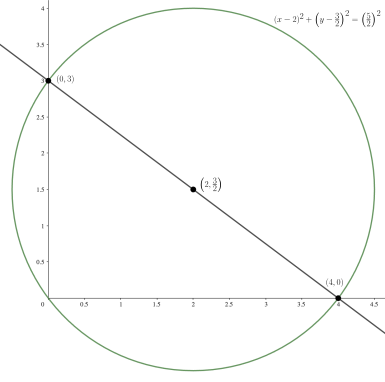
\includegraphics[width=0.5\textwidth]{varilla.png}
    \captionof{figure}{Varilla de \(5\) metros con centro geométrico en \((2, \frac{3}{2})\).}
    \label{fig:varilla}
\end{center}
\vspace*{1em}

Con los extremos de la varilla identificados, se puede plantear una parametrización de la varilla. Una parametrización común para un segmento de recta es plantear la ecuación de la recta que pasa por los dos puntos y luego expresarla en función de un parámetro \(t\) que tome el rol del eje \(x\). Para plantear la ecuación de la recta, se calcula la pendiente,
\[m = \frac{y_2 - y_1}{x_2 - x_1} = \frac{0 - 3}{4 - 0} = -\frac{3}{4},\]
y se usa la fórmula punto-pendiente para plantear la ecuación de la recta:
\[y - y_1 = m(x - x_1) \implies y = -\frac{3}{4}x + 3.\]
Con eso, si se toma \(t = x\), se puede parametrizar la varilla como
\[\bvec{r}(t) = \begin{pmatrix}
    t \\
    -\frac{3}{4}t + 3
\end{pmatrix}\]
donde \(t\) varía en el intervalo \([0, 4]\). Una forma fácil de verificar la parametrización es reemplazar los extremos de la varilla en la ecuación de la recta para ver si se obtienen los puntos correctos.\\

Habiendo formulado la parametrización de la varilla, se puede plantear la integral de la masa de la varilla como
\[m = \int_{0}^{4} \rho(\bvec{r}(t)) \norm{\bvec{r}'(t)} \: \mathrm{d}t.\]
Para evaluar la integral, se necesita calcular \(\rho(\bvec{r}(t))\) y \(\norm{\bvec{r}'(t)}\). Para el primer término, se tiene que
\[\rho(\bvec{r}(t)) = x^2 + 2y^2 = t^2 + 2\left(-\frac{3}{4}t + 3\right)^2.\]
Para el segundo término, se tiene que
\[\norm{\bvec{r}'(t)} = \norm{\begin{pmatrix}
    1 \\
    -\frac{3}{4}
\end{pmatrix}} = \sqrt{1 + \left(-\frac{3}{4}\right)^2} = \frac{5}{4} \: \text{m}.\]
donde ese valor está medido en metros. Con eso, se puede plantear la integral de la masa de la varilla como
\begin{align*}
    m &= \int_{0}^{4} \rho(\bvec{r}(t)) \norm{\bvec{r}'(t)} \: \mathrm{d}t \\
    &= \int_{0}^{4} \left(t^2 + 2\left(-\frac{3}{4}t + 3\right)^2\right) \cdot \frac{5}{4} \: \mathrm{d}t \\
    &= \frac{5}{4} \int_{0}^{4} t^2 + 2\left(-\frac{3}{4}t + 3\right)^2 \: \mathrm{d}t \\
    &= \frac{5}{4} \int_{0}^{4} t^2 + 2\left(\frac{9}{16}t^2 - \frac{9}{2}t + 9\right) \: \mathrm{d}t \\
    &= \frac{5}{4} \int_{0}^{4} t^2 + \frac{9}{8}t^2 - 9t + 18 \: \mathrm{d}t \\
    &= \frac{5}{4} \int_{0}^{4} \frac{17}{8}t^2 - 9t + 18 \: \mathrm{d}t \\
    &= \frac{5}{4} \left. \left(\frac{17}{24}t^3 - \frac{9}{2}t^2 + 18t\right) \right\vert_{0}^{4} \\
    &= \frac{5}{4} \left(\frac{17}{24} \cdot 4^3 - \frac{9}{2} \cdot 4^2 + 18 \cdot 4\right) \\
    m &= \frac{170}{3} \: \text{kg}.
\end{align*}

Con eso, se llega a la conclusión:
\begin{gbox}
    La masa de la varilla es de \(\frac{170}{3} \: \text{kg}\).
\end{gbox}
\end{problema}


\section{Integrales de superficie}

\begin{problema}[Área de helicoide]
    
    (1 punto) Considere la región \(R\) definida en coordenadas polares como \[R = \{(\theta, r) \colon 0 \leq \theta \leq 2\uppi \ \land \ 0 \leq r \leq 1\}.\] Halle el área de \(\bvec{F}\colon R\to \mathbb{R}^3\), que es la helicoide dada por \[\begin{cases}
        x = r\cos\theta, \\
        y = r\sin\theta, \\
        z = \theta.
    \end{cases}\]

\tcblower
\textbf{Solución:}\\

Note que la helicoide es una superficie parametrizada por \(\bvec{F}\colon R \to \mathbb{R}^3\), donde \(R\) es la región dada en coordenadas polares. Para hallar el área \(A\) de la superficie recuerde que, por definición, esta dada por la siguiente integral:
\[A = \int_{R} \norm{\bvec{F}_r \times \bvec{F}_\theta} \: \mathrm{d}A.\]
donde los vectores \(\bvec{F}_r\) y \(\bvec{F}_\theta\) hacen referencia a
\[\bvec{F}_r = \parder[x][r](r, \theta) \uvec{i} + \parder[y][r](r, \theta) \uvec{j} + \parder[z][r](r, \theta) \uvec{k} \quad \text{y} \quad \bvec{F}_\theta = \parder[x][\theta](r, \theta) \uvec{i} + \parder[y][\theta](r, \theta) \uvec{j} + \parder[z][\theta](r, \theta) \uvec{k}.\]
Recuerde también que una simplificación de la fórmula dada, resultante de extender el producto cruz y expresar su norma, es
\[A = \int_{R} \sqrt{\left(\parder[(x, y)][(r, \theta)]\right)^2 + \left(\parder[(y, z)][(r, \theta)]\right)^2 + \left(\parder[(x, z)][(r, \theta)]\right)^2} \: \mathrm{d}A.\]
Hasta ahora, lo anterior es válido para cualquier superficie parametrizada. Es decir, todo lo dicho sobre este problema hasta este punto es un recordatorio de conocimientos que ya deberían tener presentes. \\

Para hallar el área de la helicoide, se calculan los jacobianos de la fórmula con base en la parametrización dada. En particular, para el primer jacobiano, se tiene que
\begin{align*}
    \parder[(x, y)][(r, \theta)] &= \begin{vmatrix}
        \dparder[x][r] & \dparder[x][\theta] \\
        \dparder[y][r] & \dparder[y][\theta]
    \end{vmatrix} \\
    &= \parder[x][r] \cdot \parder[y][\theta] - \parder[x][\theta] \cdot \parder[y][r] \\
    &= \cos\theta \cdot r\cos\theta - \sin\theta \cdot r(-\sin\theta)\\
    &= r\cos^2\theta + r\sin^2\theta \\
    &= r ( \cos^2\theta + \sin^2\theta ) \\
    &= r.
\end{align*}
Para el segundo jacobiano, se tiene que
\begin{align*}
    \parder[(y, z)][(r, \theta)] &= \begin{vmatrix}
        \dparder[y][r] & \dparder[y][\theta] \\
        \dparder[z][r] & \dparder[z][\theta]
    \end{vmatrix} \\
    &= \parder[y][r] \cdot \parder[z][\theta] - \parder[y][\theta] \cdot \parder[z][r] \\
    &= \sin\theta \cdot 1 - r\cos\theta \cdot 0 \\
    &= \sin\theta.
\end{align*}
Para el tercer jacobiano, se tiene que
\begin{align*}
    \parder[(x, z)][(r, \theta)] &= \begin{vmatrix}
        \dparder[x][r] & \dparder[x][\theta] \\
        \dparder[z][r] & \dparder[z][\theta]
    \end{vmatrix} \\
    &= \parder[x][r] \cdot \parder[z][\theta] - \parder[x][\theta] \cdot \parder[z][r] \\
    &= \cos\theta \cdot 1 - r\sin\theta \cdot 0 \\
    &= \cos\theta.
\end{align*}

Reemplazando esos jacobianos en la fórmula del área, se plantea el área de la helicoide como
\begin{align*}
    A &= \int_{R} \sqrt{\left(\parder[(x, y)][(r, \theta)]\right)^2 + \left(\parder[(y, z)][(r, \theta)]\right)^2 + \left(\parder[(x, z)][(r, \theta)]\right)^2} \: \mathrm{d}A \\
    &= \int_{0}^{2\uppi} \int_{0}^{1} \sqrt{r^2 + \sin^2\theta + \cos^2\theta} \: \mathrm{d}r \: \mathrm{d}\theta \\
    &= \int_{0}^{2\uppi} \int_{0}^{1} \sqrt{r^2 + 1} \: \mathrm{d}r \: \mathrm{d}\theta.
\end{align*}
Donde la región de integración está dada por el enunciado del problema. \\

La integral resultante consiste de una suma de cuadrados dentro de un radical. Por ende, es razonable optar por sustitución trigonométrica para resolverla. En particular, realizo la sustitución \(r = \tan u\), de modo que \(\mathrm{d}r = \sec^2 u \: \mathrm{d}u\). Los límites se actualizan acorde: para el límite inferior, se tiene que \(u = \arctan(0) = 0\), y para el límite superior, se tiene que \(u = \arctan(1) = \frac{\uppi}{4}\). Con eso, la integral se convierte en
\begin{align*}
    A &= \int_{0}^{2\uppi} \int_{0}^{1} \sqrt{r^2 + 1} \: \mathrm{d}r \: \mathrm{d}\theta \\
    &= \int_{0}^{2\uppi} \: \mathrm{d}\theta \int_{0}^{\frac{\uppi}{4}} \sqrt{\tan^2 u + 1} \cdot \sec^2 u \: \mathrm{d}u \\
    &= \theta \vert_{0}^{2\uppi} \int_{0}^{\frac{\uppi}{4}} \sqrt{\sec^2 u} \cdot \sec^2 u \: \mathrm{d}u \\
    &= 2\uppi \int_{0}^{\frac{\uppi}{4}} \sec^3 u \: \mathrm{d}u.
\end{align*}
La resolución analítica de la integral indefinida de secante cúbica se realizó en el segundo ejercicio. Se obtuvo que
\[\int \sec^3 u \: \mathrm{d}u = \frac{1}{2} \left( \sec u \tan u + \ln \left| \sec u + \tan u \right| \right) + C.\]
Reemplazando eso en la integral de área, se obtiene
\begin{align*}
    A &= 2\uppi \int_{0}^{\frac{\uppi}{4}} \sec^3 u \: \mathrm{d}u \\
    &= 2\uppi \left. \left( \frac{1}{2} \left( \sec u \tan u + \ln \left| \sec u + \tan u \right| \right) \right) \right\vert_{0}^{\frac{\uppi}{4}} \\
    &= 2\uppi \left( \frac{1}{2} \left( \sec\left(\frac{\uppi}{4}\right) \tan\left(\frac{\uppi}{4}\right) + \ln \left| \sec\left(\frac{\uppi}{4}\right) + \tan\left(\frac{\uppi}{4}\right) \right| \right) - \frac{1}{2} \left( \sec(0) \tan(0) + \ln \left| \sec(0) + \tan(0) \right| \right) \right) \\
    &= 2\uppi \left( \frac{1}{2} \left( \sqrt{2} \cdot 1 + \ln \left| \sqrt{2} + 1 \right| \right) - \frac{1}{2} \left( 1 \cdot 0 + \ln \left| 1 + 0 \right| \right) \right) \\
    &= 2\uppi \left( \frac{1}{2} \left( \sqrt{2} + \ln \left( \sqrt{2} + 1 \right) \right) - \frac{1}{2} \left( 0 + 0 \right) \right) \\
    &= \uppi \left( \sqrt{2} + \ln \left( \sqrt{2} + 1 \right) \right).
\end{align*}
Con ese resultado, es posible concluir que
\begin{gbox}
    El área de la helicoide es de \(\uppi \left( \sqrt{2} + \ln \left( \sqrt{2} + 1 \right) \right)\) unidades cuadradas.
\end{gbox}






\end{problema}

\end{document}
